QA is one of the most widely used tasks for evaluating the performance of RAG systems. To systematically assess the effectiveness of RAG and GraphRAG on general QA settings, we evaluate representative methods on widely used datasets and follow standard metrics used in prior work.

\subsection{Datasets and Evaluation Metrics}
% \vspace{-0.1in}
To comprehensively evaluate the performance of GraphRAG on general QA tasks, we select four widely used datasets that cover different perspectives. For the single-hop QA task, we select the Natural Questions (NQ) dataset~\cite{kwiatkowski2019natural}. 
For the multi-hop QA task, we select HotPotQA~\cite{yang2018hotpotqa} and MultiHop-RAG~\cite{tang2024multihop} datasets. 
The MultiHop-RAG dataset categorizes queries into four types: Inference, Comparison, Temporal, and Null queries. To further analyze the performance of RAG and GraphRAG at a finer granularity, we also include NovelQA~\cite{wang2024novelqa}, which contains 21 different types of queries. For more details, please refer to Appendix~\ref{app:qa_dataset}.
We use Precision (P), Recall (R), and F1-score as evaluation metrics for the NQ and HotPotQA datasets, while accuracy is used for the MultiHop-RAG and NovelQA datasets following their original papers.
\begin{table}[!htb]
\vspace{-0.05in}
\caption{Performance comparison (\%) on NQ and Hotpot.}
\label{tab:nq_llama8b}
\centering
\vspace{-0.1in}
\resizebox{\linewidth}{!}{
\begin{tabular}{l|ccc|ccc}
\toprule
\multirow{2}{*}{\textbf{Method}} 
& \multicolumn{3}{c|}{\textbf{NQ}} 
& \multicolumn{3}{c}{\textbf{Hotpot}} \\
\cmidrule{2-7}
& P & R & F1 & P & R & F1 \\
\midrule
RAG                        
& \textbf{71.70} & \textbf{63.93} & \textbf{64.78} 
& 62.32 & 60.47 & 60.04 \\

RaptorRAG
&66.06	&59.56	&60.04
&63.81	&61.46	&61.31 \\

KG-GraphRAG (Triplets only) 
& 40.09 & 33.56 & 34.28 
& 26.88 & 24.81 & 25.02 \\

KG-GraphRAG (Triplets+Text) 
& 58.36 & 48.93 & 50.27 
& 45.22 & 42.85 & 42.60 \\

Community-GraphRAG (Local)  
& \underline{69.48} & \underline{62.54} & \underline{63.01} 
& \underline{64.14} & \underline{62.08} & \underline{61.66} \\

Community-GraphRAG (Global) 
& 60.76 & 54.99 & 54.48 
& 45.72 & 47.60 & 45.16 \\

HippoRAG2 
& 67.25 & 60.42 & 61.03 
& \textbf{65.31} & \textbf{63.26} & \textbf{63.01} \\
\bottomrule
\end{tabular}
}
\vspace{-0.2in}
\end{table}


\begin{table}[htb]
\caption{Performance comparison (\%) on the MultiHop-RAG.}
\label{tab:multihop_llama8b}
\centering
\vspace{-0.1in}
\resizebox{\linewidth}{!}{
\begin{tabular}{l|ccccc}
\toprule
\textbf{Method} 
& \textbf{Inference} 
& \textbf{Comparison} 
& \textbf{Null} 
& \textbf{Temporal} 
& \textbf{Overall} \\
\midrule
RAG                        
& \textbf{92.16} & 57.59 & 96.01 & 30.70 & 67.02 \\

RaptorRAG
&\underline{91.91}	&55.26	&{90.03}	&45.28	&68.78 \\

KG-GraphRAG (Triplets only) 
& 55.76 & 22.55 & \textbf{98.67} & 18.70 & 41.24 \\

KG-GraphRAG (Triplets+Text) 
& 67.40 & 34.70 & \underline{97.34} & 17.15 & 48.51 \\

Community-GraphRAG (Local)  
& 86.89 & \underline{60.63} & 80.07 & \underline{50.60} & \underline{69.01} \\

Community-GraphRAG (Global) 
& 89.34 & \textbf{64.02} & 19.27 & \textbf{53.34} & 64.40 \\

HippoRAG2 
& 91.54 & 58.41 &85.71 & 49.91 & \textbf{70.27} \\
\bottomrule
\end{tabular}
}
\vspace{-0.1in}
\end{table}


\begin{table*}[!htb]
\caption{Performance comparison (\%) on the NovelQA dataset.}
\label{tab:novelqa}
\vspace{-0.1in}
\resizebox{\linewidth}{!}{
\begin{tabular}{ccccccccc|ccccccccc}
\toprule
\multicolumn{1}{l}{} 
& \multicolumn{8}{c|}{\textbf{RAG}} 
& \multicolumn{9}{c}{\textbf{RaptorRAG}} \\ 
\midrule
\multicolumn{1}{l}{} 
& chara & mean & plot & relat & settg & span & times & avg
& \multicolumn{1}{l}{} & chara & mean & plot & relat & settg & span & times & avg \\

mh & 68.75 & 52.94 & 58.33 & 75.28 & 92.31 & 64.00 & 33.96 & 47.34
   & mh & 60.42 & 70.59 & 63.89 & 65.17 & 92.31 & 52 & 38.24 & 48.17 \\
sh & 69.08 & 62.86 & 66.11 & 75.00 & 78.35 & - & - & 68.73
   & sh & 66.45 & 58.57 & 65.27 & 62.50 & 74.23 & - & - & 66.25 \\
dtl & 64.29 & 45.51 & 78.57 & 10.71 & 83.78 & - & - & 55.28
    & dtl & 62.86 & 48.88 & 80.36 & 28.57 & 78.38 & - & - & 57.72 \\
avg & 67.78 & 50.57 & 67.37 & 60.80 & 80.95 & 64.00 & 33.96 & 57.12
    & avg & 64.44 & 52.83 & 67.67 & 56.80 & 76.87 & 52 & 38.24 & 57.12 \\

\midrule
\multicolumn{1}{l}{} 
& \multicolumn{8}{c|}{\textbf{KG-GraphRAG (Triplets+Text)}} 
& \multicolumn{9}{c}{\textbf{Community-GraphRAG (Local)}} \\ 
\midrule
\multicolumn{1}{l}{} 
& chara & mean & plot & relat & settg & span & times & avg
& \multicolumn{1}{l}{} & chara & mean & plot & relat & settg & span & times & avg \\

mh & 52.08 & 52.94 & 44.44 & 55.06 & 69.23 & 64.00 & 28.61 & 38.37
   & mh & 68.75 & 64.71 & 55.56 & 67.42 & 92.31 & 52.00 & 35.83 & 47.01 \\
sh & 36.84 & 45.71 & 40.17 & 87.50 & 36.08 & - & - & 39.93
   & sh & 59.87 & 58.57 & 65.69 & 87.50 & 64.95 & - & - & 63.43 \\
dtl & 38.57 & 30.90 & 42.86 & 21.43 & 32.43 & - & - & 33.60
    & dtl & 54.29 & 37.64 & 62.50 & 25.00 & 70.27 & - & - & 46.88 \\
avg & 40.00 & 36.23 & 41.09 & 49.60 & 38.10 & 64.00 & 28.61 & 37.80
    & avg & 60.00 & 44.91 & 64.05 & 59.20 & 68.71 & 52.00 & 35.83 & 53.03 \\

\midrule
\multicolumn{1}{l}{} 
& \multicolumn{8}{c|}{\textbf{Community-GraphRAG (Global)}} 
& \multicolumn{9}{c}{\textbf{HippoRAG2}} \\ 
\midrule
\multicolumn{1}{l}{} 
& chara & mean & plot & relat & settg & span & times & avg
& \multicolumn{1}{l}{} & chara & mean & plot & relat & settg & span & times & avg \\

mh & 54.17 & 58.82 & 55.56 & 56.18 & 53.85 & 68 & 20.59 & 34.39
   & mh & 58.33 & 64.71 & 66.67 & 69.66 & 92.31 & 48 & 37.17 & 47.84 \\
sh & 45.39 & 50.00 & 55.65 & 87.50 & 38.14 & - & - & 49.65
   & sh & 65.79 & 65.71 & 64.44 & 62.50 & 72.16 & - & - & 66.25 \\
dtl & 28.57 & 29.78 & 32.14 & 87.50 & 40.54 & - & - & 30.89
    & dtl & 60.00 & 48.88 & 69.64 & 28.57 & 81.08 & - & - & 55.83 \\
avg & 42.59 & 36.98 & 51.66 & 52.00 & 40.14 & 68 & 20.59 & 39.17
    & avg & 62.96 & 54.34 & 65.56 & 60.00 & 76.19 & 48 & 37.17 & 56.54 \\

\bottomrule
\end{tabular}
}
\vspace{-0.1in}
\end{table*}



% \vspace{-0.1in}


% \yu{Do we need to mention how to calculate accuracy, e.g., LLM-as-judger?}
% \vspace{-0.05in}
\subsection{QA Main Results}
\label{sec:qa_result}
% \vspace{-0.05in}
We first compare the vanilla versions of RAG and GraphRAG variants. 
Unless otherwise specified, we report {main-paper results using Llama-3.1-8B-Instruct. {Results using Llama-3.1-70B-Instruct are deferred to the Appendix~\ref{app:moreqa}.
Results on NQ and HotPotQA are shown in Table~\ref{tab:nq_llama8b}, and results on MultiHop-RAG are shown in Table~\ref{tab:multihop_llama8b}. 
Due to space constraints, we report partial results on NovelQA in Table~\ref{tab:novelqa}, with the full breakdown provided in Appendix~\ref{app:moreqa}.
We summarize key observations below:
\begin{enumerate}[leftmargin=*, itemsep=0pt, parsep=0pt]
    \item \textbf{RAG excels on detailed single-hop queries.} 
    RAG achieves strong performance on the single-hop benchmark NQ and on the single-hop (sh) and detail-oriented (dtl) subsets of NovelQA (Tables~\ref{tab:nq_llama8b} and~\ref{tab:novelqa}).
    \item \textbf{GraphRAG methods (e.g., HippoRAG2 and Community-GraphRAG (Local)) excel on multi-hop queries.} 
    They perform best on multi-hop QA benchmarks (HotPotQA and MultiHop-RAG) and remain competitive on the multi-hop (mh) subset of NovelQA (Tables~\ref{tab:nq_llama8b},~\ref{tab:multihop_llama8b}, and~\ref{tab:novelqa}).
    \item \textbf{Community-GraphRAG (Global) often struggles on QA.} 
    Global search retrieves high-level community summaries, which can lose fine-grained evidence and hurt detail-centric QA, as reflected on detail-oriented subsets in NovelQA. It also performs poorly on Null queries in MultiHop-RAG (ideally answered as \texttt{insufficient information}), suggesting increased hallucination risk. However, summary-level retrieval can be beneficial for Comparison and Temporal queries in MultiHop-RAG which require global information.
    
    \item \textbf{KG-based GraphRAG generally underperforms on QA due to limited graph coverage.} 
    KG-GraphRAG retrieves evidence primarily from extracted entities and relations, which can be incomplete and omit answer-critical information. In Appendix~\ref{app:sec:retrieve}, we show that only about 65.8\% of answer entities appear in the constructed KG for HotPotQA and 65.5\% for NQ, highlighting the sensitivity of KG-based retrieval to graph construction quality.
    
    % \yu{maybe can inspire future research on better KG construction method?}
\end{enumerate}
% \vspace{-0.1in} 
We further provide case studies in Appendix~\ref{app:sec:case}.

\begin{figure}[!htb]
 \vspace{-0.1in}
    \centering
    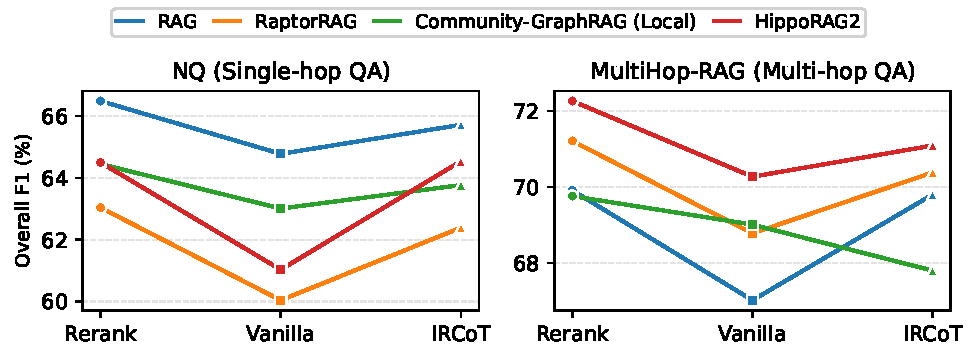
\includegraphics[width=\linewidth]{figures/rerank_and_ircot.pdf}
    \vspace{-0.1in}
    \caption{
        Overall QA performance (F1) under different inference strategies on
        NQ and MultiHop-RAG.
    }
    \label{fig:rerank_and_ircot}
        \vspace{-0.1in}
\end{figure}

\vspace{-0.1in}
\subsection{QA with Reranking and Iterative Retrieval}
In addition to vanilla retrieval, we examine the impact of \emph{reranking} and \emph{iterative retrieval} on QA performance. We conduct experiments on \textbf{NQ} and \textbf{MultiHop-RAG}, representing single-hop and multi-hop QA scenarios, respectively. Figure~\ref{fig:rerank_and_ircot} summarizes overall performance under different inference strategies.

Across both datasets, reranking and iterative retrieval generally improve performance for all methods compared to vanilla inference, indicating that inference-time enhancements provide gains beyond the underlying retrieval architecture. On \textbf{NQ}, both reranking and iterative retrieval (IRCoT) yield consistent improvements, suggesting that such refinements can be beneficial even for predominantly single-hop QA. Importantly, our earlier conclusion remains unchanged: RAG still performs better on single-hop, detail-oriented questions, even when equipped with reranking or iterative retrieval. On the \textbf{MultiHop-RAG} benchmark, the gains from inference-time strategies are more pronounced. Both reranking and IRCoT lead to larger absolute improvements than on NQ, highlighting the value of progressive evidence refinement in multi-hop settings. Under these enhanced inference strategies, GraphRAG methods also typically outperform RAG. One exception is Community-GraphRAG (Local) with IRCoT, which exhibits notably low performance on \texttt{NULL} queries, despite improvements on other categories. This observation remains consistent with our main findings.

Overall, reranking and iterative retrieval are complementary to both RAG and GraphRAG, and are particularly important for multi-hop QA. Detailed results are reported in Appendix~\ref{app:sec:iterative_retrieval} and ~\ref{app:sec:reranking}.







\begin{figure}[htb]
    \centering
    % ---------- Row 1 ----------
    \begin{subfigure}[b]{0.35\columnwidth}
        \centering
        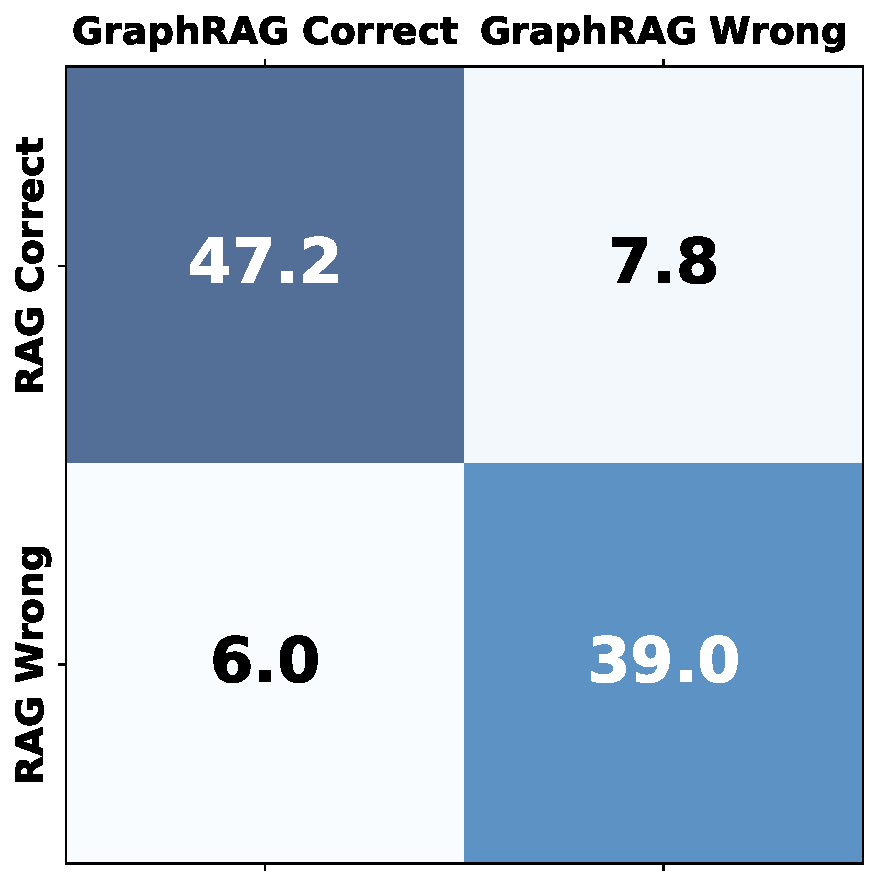
\includegraphics[width=\textwidth]{figures/NQ-8B-overlap.pdf}
        \caption{NQ}
    \end{subfigure}
   \hspace{0.01\textwidth}
    \begin{subfigure}[b]{0.35\columnwidth}
        \centering
        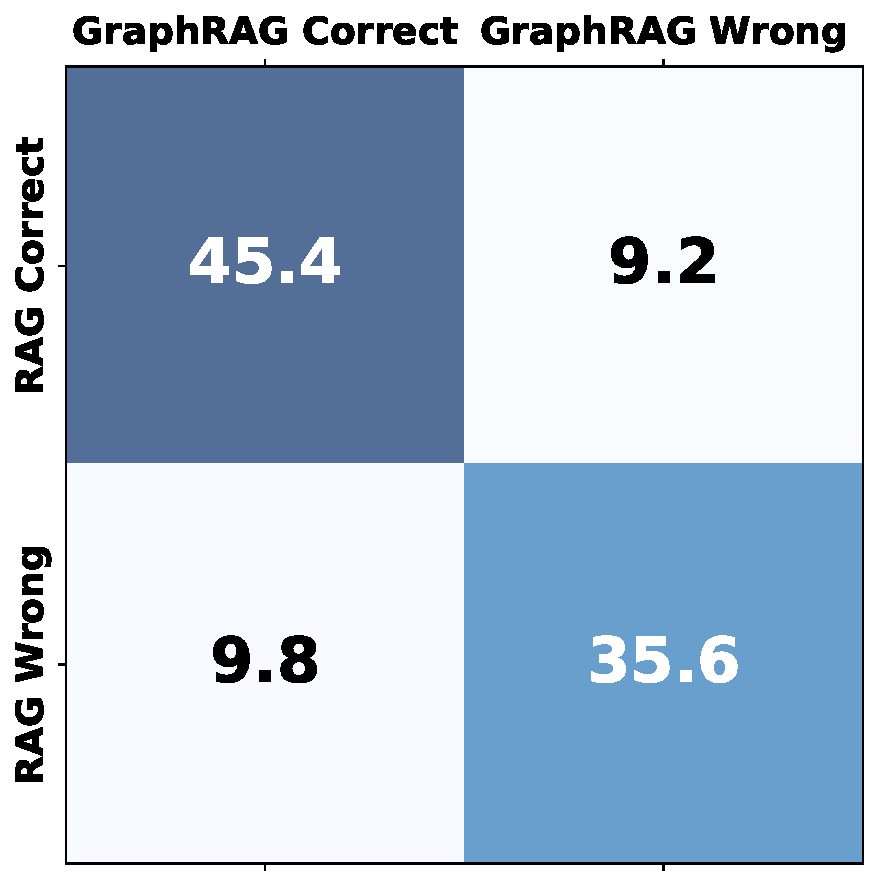
\includegraphics[width=\textwidth]{figures/hotpot-8B-overlap.pdf}
        \caption{HotpotQA}
    \end{subfigure}

    \vspace{0.1cm}

    % ---------- Row 2 ----------
    \begin{subfigure}[b]{0.35\columnwidth}
        \centering
        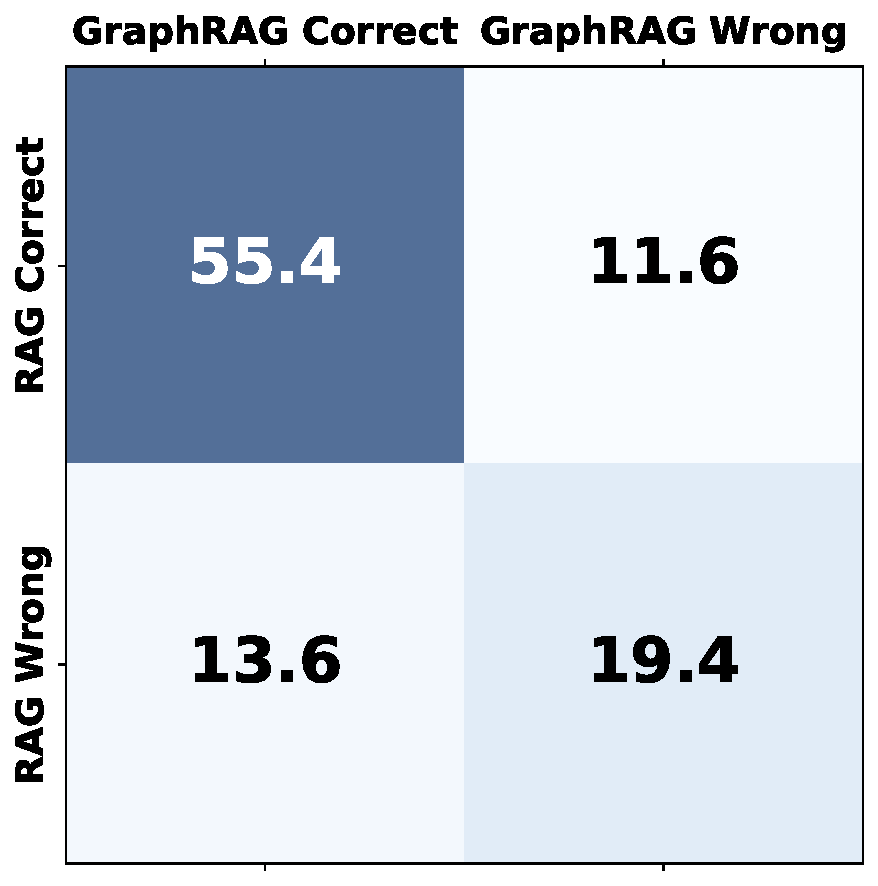
\includegraphics[width=\textwidth]{figures/news-8B-overlap.pdf}
        \caption{MultiHop-RAG}
    \end{subfigure}
    \hspace{0.01\textwidth}
    \begin{subfigure}[b]{0.35\columnwidth}
        \centering
        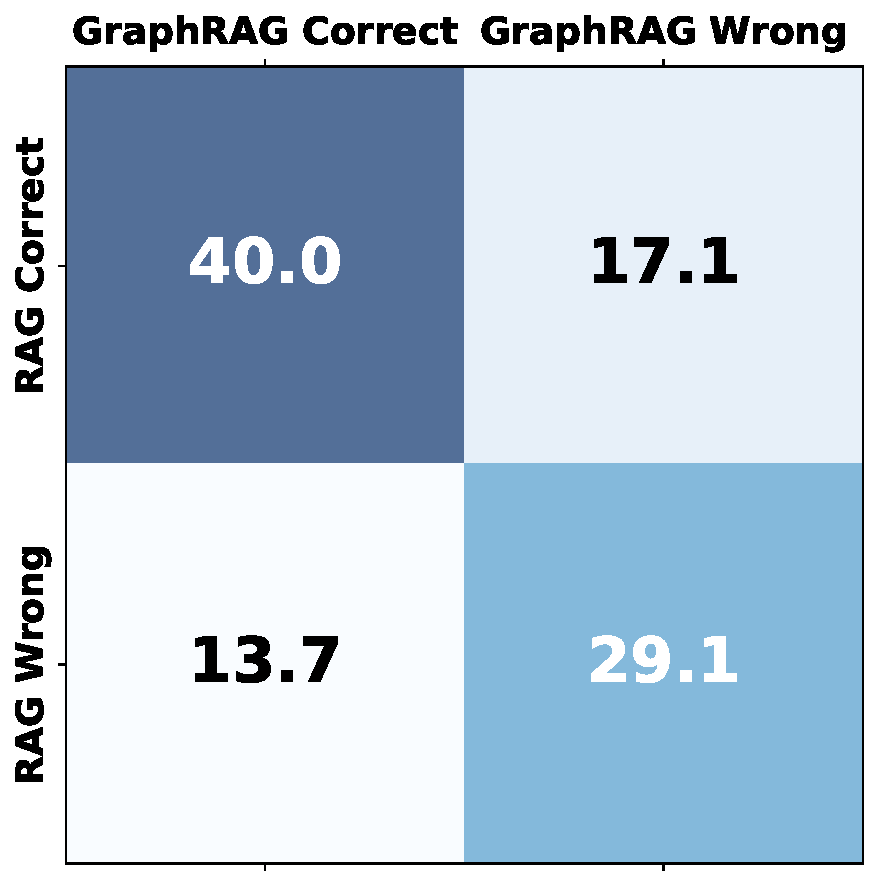
\includegraphics[width=\textwidth]{figures/NovelQA-8B-overlap.pdf}
        \caption{NovelQA}
    \end{subfigure}
    \vspace{-0.1in}
    \caption{Confusion matrices comparing GraphRAG and RAG correctness across datasets using Llama~3.1-8B.}
    \label{fig:confusion}
        \vspace{-0.2in}
\end{figure}


% \vspace{-0.1in}
\subsection{Comparative QA Analysis}
In this section, we provide a detailed comparison of RAG and GraphRAG, with a focus on their respective strengths and weaknesses. Unless otherwise specified, we consider vanilla RAG and Community-GraphRAG (Local), and refer to the latter simply as GraphRAG, as it exhibits performance comparable to RAG in our experiments. 
We partition all queries into four categories: {\bf (1)} queries correctly answered by both methods, {\bf (2)} queries correctly answered only by RAG (RAG-only), {\bf (3)} queries correctly answered only by GraphRAG (GraphRAG-only), and {\bf (4)} queries incorrectly answered by both methods.


The confusion matrices representing these four groups using the Llama 3.1-8B model are shown in Figure~\ref{fig:confusion}. Notably, the proportions of queries correctly answered exclusively by GraphRAG and RAG are significant. For example, 13.6\% of queries are GraphRAG-only, while 11.6\% are RAG-only on MultiHop-RAG dataset. This phenomenon highlights the complementary properties of RAG and GraphRAG.
% and each method has its own strengths and weaknesses. 
Therefore, {\it leveraging their unique advantages has the potential to improve overall performance}.



% ~\cite{lee2024hybgrag,xia2024knowledge}.

% \yu{can cite some recent hybrid method works such as "HybGRAG: Hybrid Retrieval-Augmented Generation on Textual and Relational Knowledge Bases", "Knowledge-Aware Query Expansion with Large Language Models for Textual and Relational Retrieval"



% \vspace{-0.1in}
\subsection{Improving QA Performance}
% \vspace{-0.05in}
\label{sec:improve_qa}
Building on the complementary properties of RAG and GraphRAG, we investigate the following two strategies to enhance overall QA performance.

\vspace{-0.05in}
\paragraph{Strategy 1: RAG vs. GraphRAG Selection}
In Section~\ref{sec:qa_result}, we observe that RAG generally performs well on single-hop queries and those requiring detailed information, while GraphRAG (Community-GraphRAG (Local)) excels in multi-hop queries that require reasoning. Therefore, we hypothesize that RAG is well-suited for fact-based queries, which rely on direct retrieval and detailed information, whereas GraphRAG is more effective for reasoning-based queries that involve chaining multiple facts together. Therefore, given a query, we employ a classification mechanism to determine whether it is fact-based or reasoning-based. Each query is then assigned to either RAG or GraphRAG based on the classification results. Specifically, we leverage the in-context learning ability of LLMs for classification~\cite{dong2022survey, wei2023larger}. Further details and prompts can be found in Appendix~\ref{app:selection}. In this strategy, either RAG or GraphRAG is selected for each query, and we refer to this strategy as \textbf{Selection}.

\vspace{-0.1in}
\paragraph{Strategy 2: RAG and GraphRAG Integration}
We further explore an \textbf{Integration} strategy that jointly leverages the complementary retrieval behaviors of RAG and GraphRAG. For each query, both methods retrieve relevant information in parallel, and the retrieved contexts are concatenated and fed into the generator to produce the final answer.
We evaluate the effectiveness of the two proposed strategies on all selected datasets. For MultiHop-RAG and NovelQA, we report overall accuracy, while for NQ and HotPotQA, we use F1 score as the evaluation metric. The results are summarized in Figure~\ref{fig:qa_improve} and Appendix~\ref{app:inte}.

\begin{figure*}[!htb]
    \centering
    \begin{subfigure}[b]{0.4\textwidth}
        \centering
        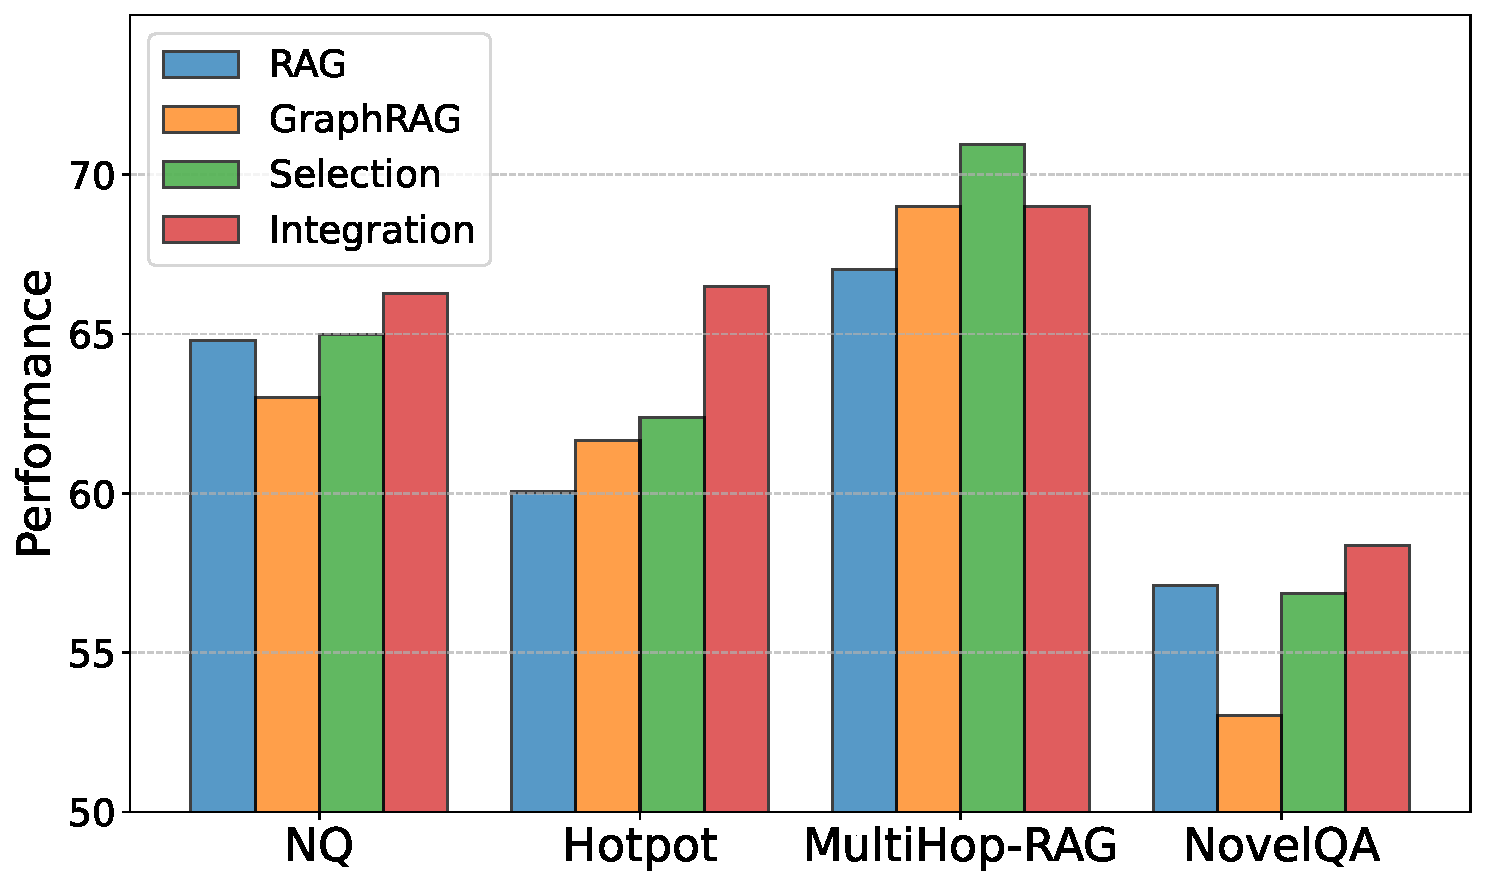
\includegraphics[width=\textwidth]{figures/qa_improvement_8B.pdf}
        \caption{Llama3.1-8B}
        \label{fig:qa_improve_8b}
    \end{subfigure}
    \hspace{0.01\textwidth}
    \begin{subfigure}[b]{0.4\textwidth}
        \centering
        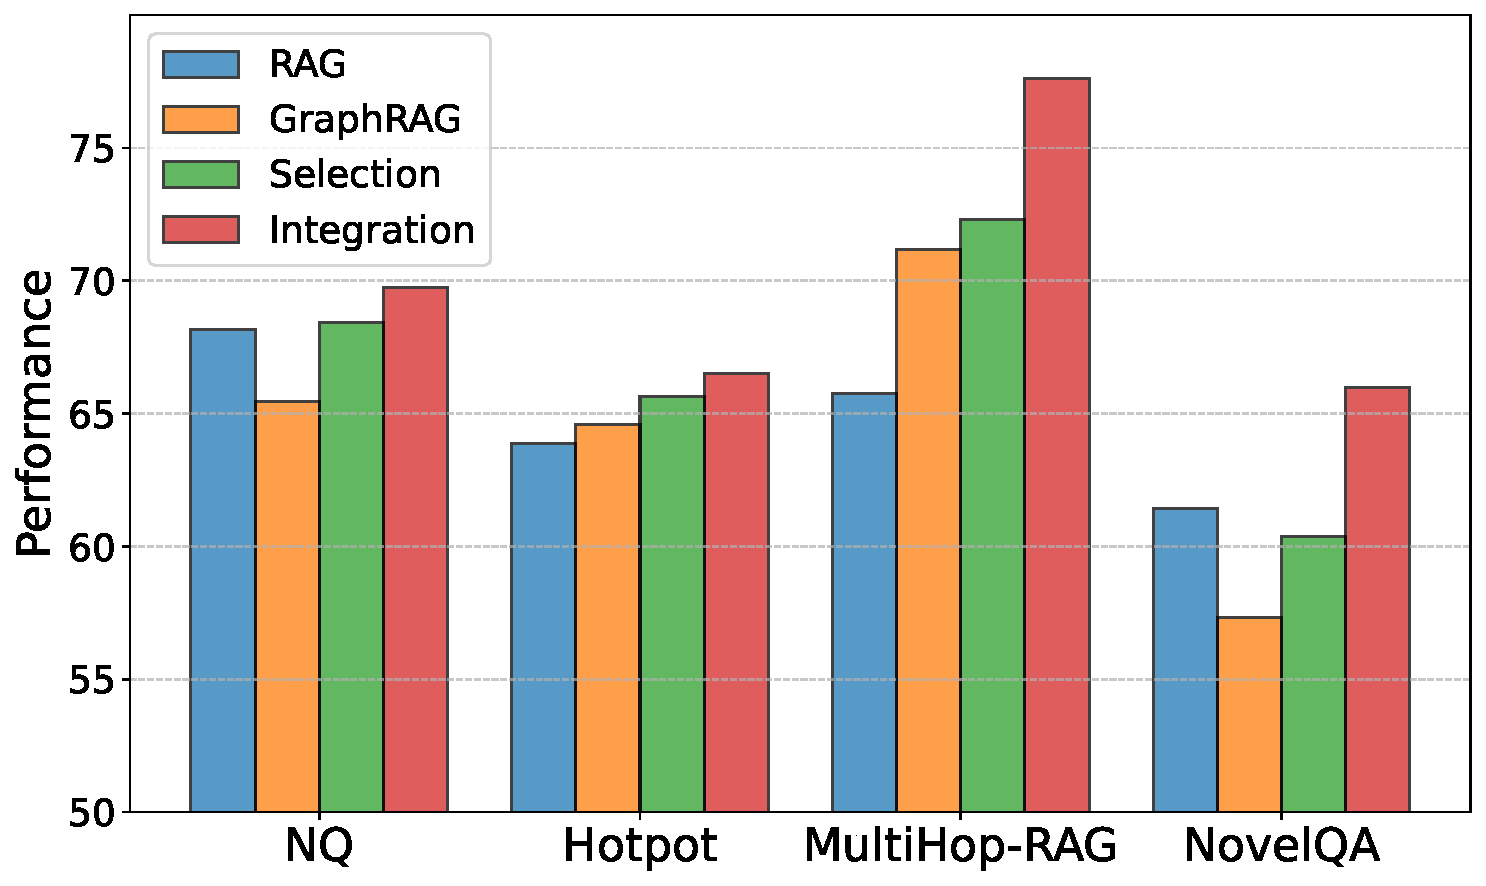
\includegraphics[width=\textwidth]{figures/qa_improvement_70B.pdf}
        \caption{Llama3.1-70B}
        \label{fig:qa_improve_70b}
    \end{subfigure}
    % \vspace{-0.1in}
    \caption{Overall QA performance comparison of different methods.}
    \label{fig:qa_improve}
    % \vspace{-0.2in}
\end{figure*}






Overall, both strategies consistently improve QA performance across datasets. For instance, on MultiHop-RAG with Llama~3.1-70B, the Selection and Integration strategies improve the best baseline by 1.1\% and 6.4\%, respectively. When comparing the two strategies, Integration generally achieves higher performance than Selection.
However, Selection processes each query using only a single method, making it more computationally efficient. In contrast, Integration requires running both RAG and GraphRAG for every query, leading to higher computational cost.

\begin{table}[!htb]
\centering
\caption{The time and storage analysis on MultiHop-RAG.}
\label{tab:time:multi}
\vspace{-0.1in}
\resizebox{\linewidth}{!}{
\begin{tabular}{c|ccc}
\hline
Method             & Construction Time (s) & Retrieval time (s) & Storage \\ \hline
RAG                & 135               & 1724          & 127MB   \\
KG-GraphRAG        & 7702              & 14434         & 117MB   \\
Community-GraphRAG & 5560              & 1249          & 165MB   \\ \hline
\end{tabular}
}
\vspace{-0.1in}
\end{table}

% \vspace{-0.1in}
\subsection{Computation and Storage Analysis}
In this subsection, we analyze the computational and storage trade-offs among RAG, KG-GraphRAG, and Community-GraphRAG. Specifically, we report construction time, retrieval latency, and storage footprint on the MultiHop-RAG dataset. The results are summarized in Table~\ref{tab:time:multi}. Results for additional datasets and tasks are provided in Appendix~\ref{app:sec:time}.
From the results, we have the following observations:
\begin{itemize}[leftmargin=1em]
\item \textbf{Construction time:} Both GraphRAG variants incur substantially higher construction cost than RAG, as they require additional graph construction and preprocessing.
\item \textbf{Retrieval time:} KG-GraphRAG exhibits the highest retrieval latency, primarily due to LLM-based entity expansion and multi-step graph traversal. In contrast, Community-GraphRAG achieves the lowest retrieval latency by relying on direct community-level matching, even outperforming vanilla RAG.
\item \textbf{Storage:} Community-GraphRAG requires the largest storage footprint, as it stores both community representations and associated summaries. KG-GraphRAG is more storage-efficient than Community-GraphRAG and RAG, reflecting a trade-off between information richness and storage cost.
\end{itemize}

We additionally report the number of retrieved tokens for each method and evaluate their performance under a fixed retrieval token budget, with detailed results provided in the Appendix~\ref{app:sec:time}.


\subsection{Graph Construction Model}
In this subsection, we analyze how graph construction quality affects GraphRAG performance. We focus on Community-GraphRAG (Local) as a representative GraphRAG variant and vary the LLM used for graph construction, while keeping the retrieval and generation components fixed. We evaluate downstream QA performance across multiple tasks and datasets, with detailed results reported in Appendix~\ref{app:graphconstruction}. Table~\ref{app:tab:cons2} summarizes results on MultiHop-RAG across different query categories.

\begin{table}[!htb] 
\centering 
\caption{Impact of graph construction models on the MultiHop-RAG dataset using Llama~3.1--70B-Instruct.} 
\label{app:tab:cons2} 
\vspace{-0.1in}
\resizebox{\linewidth}{!}{ 
\begin{tabular}{c|ccccc} \hline 
\textbf{Graph Construction} & Inference & Comparison & NULL & Temporal & Overall \\ \hline 
None (RAG) & 94.85 & 56.31 & 91.36 & 25.73 & 65.77 \\ 
GPT-4o-mini & 92.03 & 60.16 & 88.70 & 49.06 & 71.17 \\ 
GPT-4o & 93.63 & 66.59 & 81.06 & 58.49 & 75.08 \\ \hline 
\end{tabular} } 
\vspace{-0.1in}
\end{table}

We observe that stronger graph construction models consistently improve QA performance, especially on reasoning-intensive queries such as Comparison and Temporal. While omitting explicit graph construction (i.e., RAG) yields strong performance on Inference and NULL queries, it performs poorly on multi-hop reasoning tasks. In contrast, graphs constructed using more capable LLMs, such as GPT-4o, substantially improve performance on these challenging categories, leading to the highest overall accuracy.
These results indicate that GraphRAG performance is sensitive to graph construction quality. However, stronger construction models also incur higher computational cost, highlighting a trade-off between graph quality and system efficiency when selecting LLMs for graph construction.

\noindent\textbf{Summary.}
Across our QA experiments, we find that RAG and GraphRAG exhibit complementary strengths rather than a clear dominance. RAG consistently performs well on single-hop, fact-centric queries that require precise retrieval of detailed information, while GraphRAG excels on reasoning-intensive, multi-hop queries by explicitly modeling relationships among entities. However, these benefits come with different computational and storage trade-offs, and GraphRAG performance is further influenced by the quality of graph construction. Motivated by these observations, we explore selection and integration strategies that combine the strengths of both paradigms, leading to consistent improvements in overall QA performance. Together, these results suggest that effective QA systems should adaptively balance retrieval precision, reasoning capability, and system efficiency, rather than relying on a single retrieval paradigm.






